% Drawing 121/03-3 -- folder 121, batch 03, archive page 42 (PDF page 43).
% Transcription: au milieu à gauche, la tour encadrée : « $X_0 =$ » devant les cases $[\Phi_0]$, $[\Phi_1]$, $[\Phi_2]$, des flèches montant vers $X_1$ et $X_2$ ; au-dessous $\partial\Phi_1$ et $\partial\Phi_2$, la case $[(\partial_0\Phi_2)]$, $(\partial_1\Phi_2)$ et les cases $[(\partial_1\Phi_2)_0]$, $[(\partial_1\Phi_2)_1]$, avec $\Psi_0$, $\Psi_1$ et $\partial(\partial_1\Phi_2)_1$ ; de longues flèches courbes, chacune marquée d'un petit cercle, vont vers $[\Phi_0]$ et $[\Phi_1]$.
% Kind: boxed tower X_0 -> X_1 -> X_2 with ringed arrows. Method 2 (schematic redraw from the facsimile). Status: partial.
% Notes: The tower as drawn on the page, middle left: X_0 = in front of three boxes [Phi_0], [Phi_1], [Phi_2]; an arrow from [Phi_0] up to X_1 and from X_1 up to X_2; a heavy arrow from [Phi_1] up to X_1, an arrow from [Phi_2] up to X_2, and a long arrow from beside dPhi_2 up to X_1 (the attaching map dPhi_2 -> X_1, as read). Below: dPhi_1 with an arrow up to [Phi_1] (a small square drawn across its shaft), dPhi_2 with an arrow up to [Phi_2]; the box [(d_0Phi_2)] with an arrow up to dPhi_2, and an arrow towards dPhi_2 from the right, from (d_1Phi_2); (d_1Phi_2), unboxed, with arrows up to it from the boxes [(d_1Phi_2)_0] and [(d_1Phi_2)_1]; the lower edge of [(d_1Phi_2)_1] is an arrow pointing right, followed by two short strokes and Psi_1; two short strokes and Psi_0 under [(d_1Phi_2)_0]; d(d_1Phi_2)_1 with an arrow up to [(d_1Phi_2)_1] (a small square across its shaft). Arrows marked by a small ring on their shaft: dPhi_1 -> [Phi_0] (short), [(d_0Phi_2)] -> [Phi_0], [(d_1Phi_2)_0] -> [Phi_0] (long arc round the left), [(d_1Phi_2)_1] -> [Phi_1] (long arc over the top, crossing [Phi_2]), and d(d_1Phi_2)_1 -> [(d_1Phi_2)_0] (short). Boxes drawn as he drew them (the left side of [(d_1Phi_2)_0] and of [(d_1Phi_2)_1] are separate strokes, their lower edges are not closed against the sides). Still differs: free strokes placed from the 400 dpi colour crop, curved arrows drawn smooth through points read on it; what the small squares across two shafts and the two short strokes before Psi_0 and Psi_1 stand for is not read. The other three schemas of the page are relations to be set as text (given in the report of the finishing pass, scratchpad rmisc-report). Redrawn 2026-11-12 (issue 128): to check again.
% Coordinates: 1 unit = 0.84 mm = 1/100 of the crop width (bbox in page fractions: [0.15, 0.33, 0.57, 0.575]).
% Redrawn by Claude (claude-opus-5-5), issue #128, 2026-11-12; not checked by a human; not compiled (no TeX in the session).
% Rights: reproduces part of the work -- behind RENDER_TRANSCRIPTS, never published by itself.
\documentclass[tikz,border=3pt]{standalone}
\usepackage{amsmath,amssymb}
\usetikzlibrary{patterns,arrows.meta}
\tikzset{pencil/.style={black!45}, struck/.style={black!35}, mpt/.style={circle,draw,inner sep=1.3pt}, pt/.style={circle,fill,inner sep=0.9pt}, opt/.style={circle,draw,fill=white,inner sep=1.1pt}}
\begin{document}
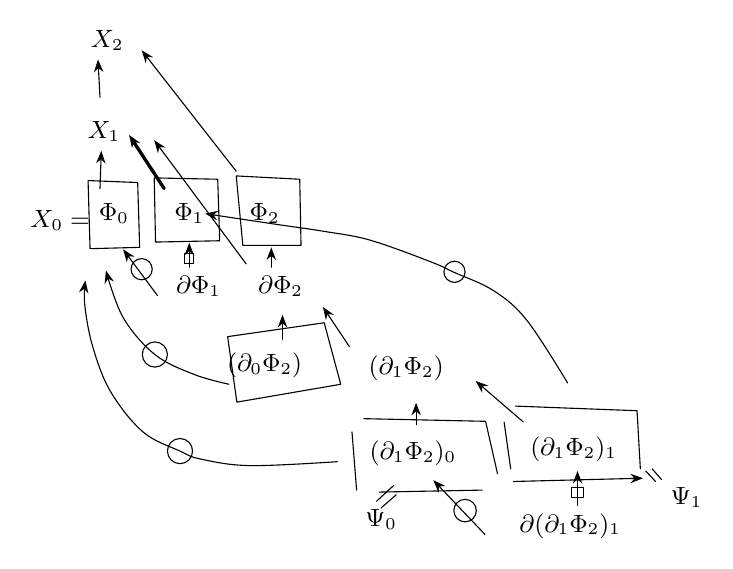
\begin{tikzpicture}[x=0.84mm,y=0.84mm,line cap=round,line join=round,font=\scriptsize]
\draw (9.0,-24.5) -- (16.5,-24.8) -- (16.8,-34.6) -- (9.3,-34.8) -- (9.0,-24.5);
\draw (19.0,-24.1) -- (28.6,-24.3) -- (28.9,-33.6) -- (19.2,-33.8) -- (19.0,-24.1);
\draw (31.4,-23.8) -- (41.0,-24.3) -- (41.2,-34.3) -- (32.4,-34.3) -- (31.4,-23.8);
\draw (30.1,-48.1) -- (44.7,-46) -- (47.2,-55.3) -- (31.5,-58) -- (30.1,-48.1);
\draw (50.7,-60.5) -- (69.1,-60.9) -- (70.9,-68.8);
\draw (48.9,-62.5) -- (49.6,-71.3);
\draw (53,-71.6) -- (68.6,-71.3);
\draw (73.6,-58.6) -- (92,-59.3) -- (92.5,-68.1);
\draw (71.9,-61.0) -- (72.9,-68.1);
\draw[-{Stealth[length=1.6mm]}] (73.3,-70.0) -- (92.9,-69.5);
\draw (93.3,-68.4) -- (94.8,-70.0);
\draw (94.3,-68.1) -- (95.7,-69.7);
\draw (52.6,-73) -- (55.2,-70.6);
\draw (53.3,-74) -- (55.6,-72);
\draw[-{Stealth[length=1.6mm]}] (10.8,-11.9) -- (10.5,-6.2);
\draw[-{Stealth[length=1.6mm]}] (10.8,-25.7) -- (11.0,-20.0);
\draw[-{Stealth[length=1.6mm]}, very thick] (20.5,-25.7) -- (15.2,-17.6);
\draw[-{Stealth[length=1.6mm]}] (31.4,-23.1) -- (17.1,-4.8);
\draw[-{Stealth[length=1.6mm]}] (32.9,-37.1) -- (19.0,-18.4);
\draw[-{Stealth[length=1.6mm]}] (24.3,-37.6) -- (24.3,-33.9);
\draw (23.6,-35.5) -- (25.0,-35.5) -- (25.0,-37.0) -- (23.6,-37.0) -- (23.6,-35.5);
\draw[-{Stealth[length=1.6mm]}] (36.7,-37.6) -- (36.7,-34.6);
\draw[-{Stealth[length=1.6mm]}] (19.5,-41.9) -- (14.3,-34.9);
\draw (17.1,-37.9) circle[radius=1.6];
\draw[-{Stealth[length=1.6mm]}] (38.4,-48.5) -- (38.4,-44.8);
\draw[-{Stealth[length=1.6mm]}] (48.5,-49.6) -- (44.5,-43.6);
\draw[-{Stealth[length=1.6mm]}] plot[smooth, tension=0.6] coordinates {(30.3,-55.3) (25,-53.8) (19.1,-50.8) (14.3,-45.2) (11.7,-38.1)};
\draw (19.1,-50.8) circle[radius=1.9];
\draw[-{Stealth[length=1.6mm]}] plot[smooth, tension=0.6] coordinates {(46.7,-67) (33.5,-67.6) (26,-66.6) (22.9,-65.4) (17.3,-62.5) (12.4,-56.4) (9.7,-49.6) (8.5,-43.3) (8.6,-39.6)};
\draw (22.9,-65.4) circle[radius=1.9];
\draw[-{Stealth[length=1.6mm]}] plot[smooth, tension=0.6] coordinates {(81.5,-55.1) (75.4,-45.7) (70.4,-41.2) (64.4,-38.4) (60.6,-36.7) (51.6,-33.5) (44.8,-32.2) (38,-31.2) (32,-30.3) (26.7,-29.5)};
\draw (64.4,-38.3) circle[radius=1.6];
\draw[-{Stealth[length=1.6mm]}] (58.6,-61.4) -- (58.6,-58.1);
\draw[-{Stealth[length=1.6mm]}] (74.8,-61.0) -- (67.6,-54.8);
\draw[-{Stealth[length=1.6mm]}] (69,-78) -- (61.2,-69.8);
\draw (66,-74.4) circle[radius=1.7];
\draw[-{Stealth[length=1.6mm]}] (83,-73.6) -- (83,-68.4);
\draw (82.1,-70.9) -- (83.9,-70.9) -- (83.9,-72.4) -- (82.1,-72.4) -- (82.1,-70.9);
\node[inner sep=1pt] at (11.9,-3.3) {\small $X_2$};
\node[inner sep=1pt] at (11.4,-17.1) {\small $X_1$};
\node[inner sep=1pt] at (4.8,-30.5) {\small $X_0 =$};
\node[inner sep=1pt] at (12.9,-29.5) {\small $\Phi_0$};
\node[inner sep=1pt] at (24.3,-29.5) {\small $\Phi_1$};
\node[inner sep=1pt] at (35.7,-29.5) {\small $\Phi_2$};
\node[inner sep=1pt] at (25.7,-40.5) {\small $\partial\Phi_1$};
\node[inner sep=1pt] at (38.1,-40.5) {\small $\partial\Phi_2$};
\node[inner sep=1pt] at (35.7,-52.4) {\small $(\partial_0\Phi_2)$};
\node[inner sep=1pt] at (57.1,-52.9) {\small $(\partial_1\Phi_2)$};
\node[inner sep=1pt] at (58.1,-65.7) {\small $(\partial_1\Phi_2)_0$};
\node[inner sep=1pt] at (82.4,-65.2) {\small $(\partial_1\Phi_2)_1$};
\node[inner sep=1pt] at (81.9,-76.7) {\small $\partial(\partial_1\Phi_2)_1$};
\node[inner sep=1pt] at (53.3,-75.8) {\small $\Psi_0$};
\node[inner sep=1pt] at (99.5,-72.4) {\small $\Psi_1$};
\end{tikzpicture}
\end{document}
